\ifx\allfiles\undefined
\documentclass[12pt, a4paper,oneside, UTF8]{ctexbook}
\usepackage[dvipsnames]{xcolor}
\usepackage{amsmath}   % 数学公式
\usepackage{amsthm}    % 定理环境
\usepackage{amssymb}   % 更多公式符号
\usepackage{graphicx}  % 插图
%\usepackage{mathrsfs}  % 数学字体
%\usepackage{newtxtext,newtxmath}
%\usepackage{arev}
\usepackage{kmath,kerkis}
\usepackage{newtxtext}
\usepackage{bbm}
\usepackage{enumitem}  % 列表
\usepackage{geometry}  % 页面调整
%\usepackage{unicode-math}
\usepackage[colorlinks,linkcolor=black]{hyperref}

\usepackage{wrapfig}


\usepackage{ulem}	   % 用于更多的下划线格式,
					   % \uline{}下划线,\uuline{}双下划线,\uwave{}下划波浪线,\sout{}中间删除线,\xout{}斜删除线
					   % \dashuline{}下划虚线,\dotuline{}文字底部加点


\graphicspath{ {flg/},{../flg/}, {config/}, {../config/} }  % 配置图形文件检索目录
\linespread{1.5} % 行高

% 页码设置
\geometry{top=25.4mm,bottom=25.4mm,left=20mm,right=20mm,headheight=2.17cm,headsep=4mm,footskip=12mm}

% 设置列表环境的上下间距
\setenumerate[1]{itemsep=5pt,partopsep=0pt,parsep=\parskip,topsep=5pt}
\setitemize[1]{itemsep=5pt,partopsep=0pt,parsep=\parskip,topsep=5pt}
\setdescription{itemsep=5pt,partopsep=0pt,parsep=\parskip,topsep=5pt}

% 定理环境
% ########## 定理环境 start ####################################
\theoremstyle{definition}
\newtheorem{defn}{\indent 定义}[section]

\newtheorem{lemma}{\indent 引理}[section]    % 引理 定理 推论 准则 共用一个编号计数
\newtheorem{thm}[lemma]{\indent 定理}
\newtheorem{corollary}[lemma]{\indent 推论}
\newtheorem{criterion}[lemma]{\indent 准则}

\newtheorem{proposition}{\indent 命题}[section]
\newtheorem{example}{\indent \color{SeaGreen}{例}}[section] % 绿色文字的 例 ,不需要就去除\color{SeaGreen}{}
\newtheorem*{rmk}{\indent \color{red}{注}}

% 两种方式定义中文的 证明 和 解 的环境:
% 缺点:\qedhere 命令将会失效【技术有限,暂时无法解决】
\renewenvironment{proof}{\par\textbf{证明.}\;}{\qed\par}
\newenvironment{solution}{\par{\textbf{解.}}\;}{\qed\par}

% 缺点:\bf 是过时命令,可以用 textb f等替代,但编译会有关于字体的警告,不过不影响使用【技术有限,暂时无法解决】
%\renewcommand{\proofname}{\indent\bf 证明}
%\newenvironment{solution}{\begin{proof}[\indent\bf 解]}{\end{proof}}
% ######### 定理环境 end  #####################################

% ↓↓↓↓↓↓↓↓↓↓↓↓↓↓↓↓↓ 以下是自定义的命令  ↓↓↓↓↓↓↓↓↓↓↓↓↓↓↓↓

% 用于调整表格的高度  使用 \hline\xrowht{25pt}
\newcommand{\xrowht}[2][0]{\addstackgap[.5\dimexpr#2\relax]{\vphantom{#1}}}

% 表格环境内长内容换行
\newcommand{\tabincell}[2]{\begin{tabular}{@{}#1@{}}#2\end{tabular}}

% 使用\linespread{1.5} 之后 cases 环境的行高也会改变,重新定义一个 ca 环境可以自动控制 cases 环境行高
\newenvironment{ca}[1][1]{\linespread{#1} \selectfont \begin{cases}}{\end{cases}}
% 和上面一样
\newenvironment{vx}[1][1]{\linespread{#1} \selectfont \begin{vmatrix}}{\end{vmatrix}}

\def\d{\textup{d}} % 直立体 d 用于微分符号 dx
\def\R{\mathbb{R}} % 实数域
\def\N{\mathbb{N}} % 自然数域
\def\C{\mathbb{C}} % 复数域
\def\Z{\mathbb{Z}} % 整数环
\def\Q{\mathbb{Q}} % 有理数域
\newcommand{\bs}[1]{\boldsymbol{#1}}    % 加粗,常用于向量
\newcommand{\ora}[1]{\overrightarrow{#1}} % 向量

% 数学 平行 符号
\newcommand{\pll}{\kern 0.56em/\kern -0.8em /\kern 0.56em}

% 用于空行\myspace{1} 表示空一行 填 2 表示空两行  
\newcommand{\myspace}[1]{\par\vspace{#1\baselineskip}}

%s.t. 用\st就能打出s.t.
\DeclareMathOperator{\st}{s.t.}

%罗马数字 \rmnum{}是小写罗马数字, \Rmnum{}是大写罗马数字
\makeatletter
\newcommand{\rmnum}[1]{\romannumeral #1}
\newcommand{\Rmnum}[1]{\expandafter@slowromancap\romannumeral #1@}
\makeatother
\begin{document}
	% \title{{\Huge{\textbf{$Real \,\, Analysis$}}}\\
		\Large{\textbf{$Measure \,\, Theory , \,\, Integration , \,\, \& \,\, Hilbert \,\, Spaces$}}\footnote{参考书籍:\\
			\hspace*{4em} \textbf{《$Real \,\, Analysis -- Measure \,\, Theroy, \,\, Integration, \,\, \& \,\, Hilbert \,\, Spaces$》--- $Elias \,\, M. \,\, Stein$} \\
			\hspace*{4em} \textbf{《$Real \,\, Analysis -- Modern \,\, Techniques \,\, and \,\, Their \,\, Applications$》--- $Gerald \,\, B. \,\, Folland$}}}
\author{$-TW-$}
\date{\today}
\maketitle                   % 在单独的标题页上生成一个标题

\thispagestyle{empty}        % 前言页面不使用页码
\begin{center}
	\Huge\textbf{序}
\end{center}


\vspace*{3em}
\begin{center}
	\large{\textbf{天道几何,万品流形先自守;}}\\
	
	\large{\textbf{变分无限,孤心测度有同伦。}}
\end{center}

\vspace*{3em}
\begin{flushright}
	\begin{tabular}{c}
		\today \\ \small{\textbf{长夜伴浪破晓梦,梦晓破浪伴夜长}}
	\end{tabular}
\end{flushright}


\newpage                      % 新的一页
\pagestyle{plain}             % 设置页眉和页脚的排版方式(plain:页眉是空的,页脚只包含一个居中的页码)
\setcounter{page}{1}          % 重新定义页码从第一页开始
\pagenumbering{Roman}         % 使用大写的罗马数字作为页码
\tableofcontents              % 生成目录

\newpage                      % 以下是正文
\pagestyle{plain}
\setcounter{page}{1}          % 使用阿拉伯数字作为页码
\pagenumbering{arabic}
\setcounter{chapter}{0}    % 设置 -1 可作为第零章绪论从第零章开始 
	\else
	\fi
	%  ############################ 正文部分
\chapter{$Integration \,\, Theory$}
\section{$The \,\, Lebesgue \,\, integral$}
	$Lebesgue$ $Integral$ 的构造可以分为三步,分别为构造下列函数的积分:
	\begin{enumerate}
		\item \textbf{Simple functions} 
	
		\item \textbf{Non-negative measurable functions}
		\begin{align}
			\int f \coloneqq \sup{\{ \int \varphi \mid \varphi \,\, simple , \,\, 0 \leq \varphi \leq f \}}
		\end{align}
	
		\item \textbf{General case}
		\begin{align}
			f &= f^{+} - f^{-} \\
			\int f &\coloneqq \int f^{+} - \int f^{-}
		\end{align}
	\end{enumerate}

\subsection{$Simple \,\, functions$}
\paragraph{定义}
	下面先给出非负简单函数在\textbf{标准形式}下的\textbf{积分}定义.
	\begin{defn}\label{def 3.1.1}
		If $\varphi$ is a non-negative simple function with \textbf{standard representation}
		\begin{align}
			\varphi(x) = \sum_{k = 1}^{M}{a_k \chi_{E_k}(x)}
		\end{align}
		We define the \underline{\textcolor{blue}{\textbf{Lebesgue integral}}} of $\varphi$ by
		\begin{align}
			\int_{\R^d}{\varphi(x) dx} = \sum_{k = 1}^{M}{a_k m(E_k)}
		\end{align}
		If $E$ is a measurable subset of $\R^d$ with finite measure, then
		\begin{align}
			\varphi(x) \chi_{E}(x) = \sum_{k = 1}^{M}{a_k \chi_{E_k}(x) \chi_{E}(x)} = \sum_{k = 1}^{M}{a_k \chi_{E_k \cap E}(x)}
		\end{align}
		is also a simple function, and define
		\begin{align}
			\int_{E}{\varphi(x) dx} = \int_{\R^d}{\varphi(x) \chi_{E}(x) dx}
		\end{align}
		
		\newpage
		\begin{rmk}
			\begin{itemize}
				\item 此处仅对\textbf{标准形式}定义了积分. 事实上,此处定义的积分与简单函数的表达形式无关(即\textcolor{red}{\textbf{Property 1.}}).
				
				\item 关于记号,当测度非常明确时,大多数情况下可简写,如
				\begin{align}
					\int_{E}{\varphi(x) dx} \,\, &\Rightarrow \,\, \int_{E}{\varphi} \\
					\int_{\R^d}{\varphi(x) dx} &\Rightarrow \,\, \int{\varphi}
				\end{align}
				当为了强调我们选择了何种测度$\mu$ 时,还可用以下的记号:
				\begin{align}
					\int_{E}{\varphi(x) d\mu(x)}
				\end{align}
			\end{itemize}
		\end{rmk}
	\end{defn}

\vspace{2em}
\paragraph{Property}
	下面给出简单函数积分的性质.
	
	\begin{enumerate}
		\item[\textcolor{red}{\textbf{Property 1.}}]\textbf{Independence of the representation}.\\
		If $\varphi = \overset{N}{\underset{k = 1}{\sum}}{a_k \chi_{E_k}}$ is any representation of $\varphi$, then
		\begin{align}
			\int \varphi = \sum_{k = 1}^{N}{a_k m(E_k)}
		\end{align}
		
		\vspace{2em}
		在证明这个性质之前,先来证明一条引理.(书\footnote{参考书籍:\textbf{《$Real \,\, Analysis -- Measure \,\, Theroy, \,\, Integration, \,\, \& \,\, Hilbert \,\, Spaces$》--- $Elias \,\, M. \,\, Stein$}}Exercises Of Chapter 2 的第1题)
		
		\begin{lemma}\label{lemma 3.1.1}
			Given a collection of sets $\{ F_k \}_{k = 1}^{n}$, there exists another collection $\{ \widetilde{F}_j \}_{j = 1}^{N}$ \\
			with $N = 2^n - 1$, so that
			\begin{align}
				(\rmnum{1})&. \hspace*{2em} \bigcup_{k = 1}^{n}{F_k} = \bigcup_{j = 1}^{N}{\widetilde{F}_j} \\
				(\rmnum{2})&. \hspace*{2em} \{ \widetilde{F}_j \}_{j = 1}^{N} \,\, are \,\, disjoint \\
				(\rmnum{3})&. \hspace*{2em} F_k = \bigcup_{\widetilde{F}_j \subset F_k}{\widetilde{F}_j}
			\end{align}
		
			\vspace{2em}
			\begin{proof}
				Consider the collection
				\begin{align}
					\mathcal{F} \coloneqq \{ \bigcup_{k = 1}^{n}{G_k} - \bigcap_{k = 1}^{n}{F_{k}^{c}} \,\, \Big| \,\, G_k \,\, denotes \,\, F_k \,\, or \,\, F_{k}^c \}
				\end{align}
			\end{proof}
		\end{lemma}
	
		\newpage	
		下面来证明原命题.
		\begin{proof}
			 According to Lemma \ref{lemma 3.1.1}, there exists another decompositon of $\overset{N}{\underset{k = 1}{\bigcup}}{E_k}$, i.e.
			 \begin{align}
			 	\bigcup_{j = 1}^{M}{\widetilde{E}_j} = \bigcup_{k = 1}^{N}{E_k}
			 \end{align}
		 	where $\{ \widetilde{E}_j \}_{j = 1}^M$ are disjoint, and for each $1 \leq k \leq M$,
		 	\begin{align}
		 		E_k = \bigcup_{\widetilde{E}_j \subset E_k}{\widetilde{E}_j}
		 	\end{align}
	 		Let
	 		\begin{align}
	 			\widetilde{a}_j \coloneqq \sum_{\widetilde{E}_j \subset E_k}{a_k}
	 		\end{align}
 			Then clearly
 			\begin{align}
 				\varphi = \sum_{j = 1}^{M}{\widetilde{a}_j \chi_{\widetilde{E}_j}}
 			\end{align}
 			Since $\{ \widetilde{E}_j \}_{j = 1}^M$ are disjoint, we get
 			\begin{align}
 				\int{\varphi} = \sum_{j = 1}^{M}{\widetilde{a}_j m(\widetilde{E}_j)} = \sum_{j = 1}^{M}{\sum_{\widetilde{E}_j \subset E_k}{a_k m(\widetilde{E}_j)}} = \sum_{k = 1}^{N}{a_k m(E_k)}
 			\end{align}
		\end{proof}
		
		\vspace{2em}
		\item[\textcolor{red}{\textbf{Property 2.}}]\textbf{Linearity}.\\
		If $\varphi$ and $\psi$ are non-negative simple, and $a , b \geq 0$, then
		\begin{align}
			\int{(a \varphi + b \psi)} = a\int{\varphi} + b\int{\psi}
		\end{align}
		
		\vspace{2em}
		\begin{proof}
			下面分为两步来证明.
			\begin{enumerate}
				\item[(a)]$\forall c \geq 0$, $\int{c \varphi} = c \int{\varphi}$.\\
				Suppose $\varphi = \overset{M}{\underset{k = 1}{\sum}}{a_k \chi_{E_k}}$, where $\{ E_k \}_{k = 1}^{M}$ are disjoint. Then
				\begin{align}
					c\varphi = \sum_{k = 1}^{M}{c a_k \chi_{E_j}}
				\end{align}
				is also a non-negative simple function. Therefore,
				\begin{align}
					\int{c\varphi} = \sum_{k = 1}^{M}{c a_k m(E_k)} = c\sum_{k = 1}^{M}{a_k m(E_k)} = c\int{\varphi}
				\end{align}
			
				\item[(b)]$\int{(\varphi + \psi)} = \int{\varphi} + \int{\psi}$.\\
				Suppose
				\begin{align}
					\varphi = \sum_{k = 1}^{M}{a_k \chi_{E_k}} , \,\, \psi = \sum_{j = 1}^{N}{b_j \chi_{F_j}}
				\end{align}
				where both $\{ E_k \}_{k = 1}^{M}$ and $\{ F_j \}_{j = 1}^{N}$ are disjoint and $\R^d = \overset{M}{\underset{k = 1}{\bigcup}}{E_k} = \overset{N}{\underset{j = 1}{\bigcup}}{F_j}$. Since
				\begin{align}
					E_k = E_k \cap \R^d = E_k \cap \bigsqcup_{j = 1}^{N}{F_j} = \bigsqcup_{j = 1}^{N}{(E_k \cap F_j)}
				\end{align}
				Then
				\begin{align}
					\varphi = \sum_{k = 1}^{M}{a_k \chi_{E_k}} = \sum_{k = 1}^{M}{a_k \chi_{\bigsqcup_{j = 1}^{N}{(E_k \cap F_j)}}} = \sum_{k = 1}^{M}{\sum_{j = 1}^{N}{a_k \chi_{E_k \cap F_j}}}
				\end{align}
				Similarly
				\begin{align}
					\psi = \sum_{j = 1}^{N}{b_j \chi_{F_j}} = \sum_{j = 1}^{N}{b_k \chi_{\bigsqcup_{k = 1}^{M}{(E_k \cap F_j)}}} = \sum_{j = 1}^{N}{\sum_{k = 1}^{M}{b_k \chi_{E_k \cap F_j}}}
				\end{align}
				Therefore
				\begin{align}
					\varphi + \psi &= \sum_{j , k}{(a_k + b_j)\chi_{E_k \cap F_j}} \\
					\int{(\varphi + \psi)} &= \sum_{j , k}{(a_k + b_j)m(E_k \cap F_j)} \\
					&= \sum_{j , k}{a_k m(E_k \cap F_j)} + \sum_{j , k}{b_j m(E_k \cap F_j)} \\
					&= \int{\varphi} + \int{\psi}
				\end{align}
			\end{enumerate}
		\end{proof}
		
		\vspace{2em}
		\item[\textcolor{red}{\textbf{Property 3.}}]\textbf{Monotonicity}.\\
		If $\varphi \leq \psi$ are non-negative and simple, then
		\begin{align}
			\int{\varphi} \leq \int{\psi}
		\end{align}
	
		\vspace{2em}
		\begin{proof}
			Suppose
			\begin{align}
				\varphi = \sum_{k = 1}^{M}{a_k \chi_{E_k}} , \,\, \psi = \sum_{j = 1}^{N}{b_j \chi_{F_j}}
			\end{align}
			where both $\{ E_k \}_{k = 1}^{M}$ and $\{ F_j \}_{j = 1}^{N}$ are disjoint. Similar to the proof in Property 2, we get
			\begin{align}
				\psi - \varphi = \sum_{j , k}{(b_j - a_k) \chi_{E_k \cap F_j}}
			\end{align}
			Since $\varphi(x) \leq \psi(x)$, $\forall x \in \R^d$, then $\psi - \varphi$ is non-negative and simple. Therefore,
			\begin{align}
				\int{(\psi - \varphi)} = \sum_{j , k}{(b_j - a_k) m(E_k \cap F_j)} \geq 0 \,\, \Rightarrow \,\, \int{\varphi} \leq \int{\psi}
			\end{align}
		\end{proof}
	
		\vspace{2em}
		\item[\textcolor{red}{\textbf{Property 4.}}]\textbf{Additivity}.\\
		If $\{ E_k \}_{k = 1}^{\infty}$ are disjoint subsets of $\R^d$ with finite measure, then
		\begin{align}
			\int_{\bigcup_{k = 1}^{\infty}{E_k}}{\varphi} = \sum_{k = 1}^{\infty}{\int_{E_k}{\varphi}}
		\end{align}
		
		\vspace{2em}
		\begin{rmk}
			首先回顾$abstract$ $measure$ 的定义.
			\begin{defn}\label{def 3.1.2}
				Let $X$ be a set and let $\mathcal{M}$ be a $\sigma-algebra$ on $X$.\\
				A \underline{\textcolor{blue}{\textbf{measure}}} on $\mathcal{M}$ is a function $\mu : \mathcal{M} \longrightarrow [0 , \infty]$, $\st$
				\begin{enumerate}
					\item[(\rmnum{1})]$\mu(\varnothing) = 0$.
					
					\item[(\rmnum{2})]If $\{ E_j \}_{j = 1}^{\infty} \subset \mathcal{M}$ are disjoint, then
					\begin{align}
						\mu(\bigcup_{j = 1}^{\infty}{E_j}) = \sum_{j = 1}^{\infty}{\mu(E_j)}
					\end{align}
				\end{enumerate}
			\end{defn}
			
			\vspace{2em}
			回到我们积分的性质上来. 下面我们将说明,对于任一给定的非负简单函数$\varphi$,将$\varphi$ 在任一可测集$A$ 上的积分看作$Lebesgue \,\, \sigma-algebra \,\, \mathcal{L}$ 上的映射,则该映射为定义在$\mathcal{L}$ 上的测度.(从而Property 4.作为测度的必要条件自然成立)
			
			\vspace{2em}
			\begin{proposition}\label{prop 3.1.1}
				For any fixed non-negative and simple function $\varphi$, the map
				\begin{align}
					\mu : \mathcal{L} &\longrightarrow [0 , \infty] \\
					A &\longmapsto \int_{A}{\varphi}
				\end{align}
				is a measure on $\mathcal{L}$.
				
				\newpage
				\begin{proof}
					Suppose $\{ A_j \}_{j = 1}^{\infty} \subset \mathcal{L}$ are disjoint, and
					\begin{align}
						\varphi = \sum_{k = 1}^{M}{a_k \chi_{E_k}} , \,\, where \,\, \{ E_k \}_{k = 1}^{M} \,\, are \,\, disjoint
					\end{align}
					Let $A = \overset{\infty}{\underset{j = 1}{\bigcup}}{A_j}$, then
					\begin{align}
						\int_{\bigcup_{j = 1}^{\infty}{A_j}}{\varphi} 
						= \int_{A}{\varphi} 
						= \int{\varphi \chi_A} 
						&= \int{(\sum_{k = 1}^{M}{a_k \chi_{E_k \cap A}})} \\
						&= \sum_{k = 1}^{M}{a_k m(E_k \cap A)} \\
						&= \sum_{k = 1}^{M}{a_k m(E_k \cap (\bigcup_{j = 1}^{\infty}{A_j}))} \\
						&= \sum_{k = 1}^{M}{a_k m(\bigsqcup_{j = 1}^{\infty}{(E_k \cap A_j)})} \\
						&= \sum_{k = 1}^{M}{a_k \sum_{j = 1}^{\infty}{m(E_k \cap A_j)}} \\
						&= \sum_{k = 1}^{M}{\sum_{j = 1}^{\infty}{a_k m(E_k \cap A_j)}}
					\end{align}
					Since positive series always converges in $[0 , \infty]$, then
					\begin{align}
						\int_{A}{\varphi} 
						= \sum_{k = 1}^{M}{\sum_{j = 1}^{\infty}{a_k m(E_k \cap A_j)}} 
						= \sum_{j = 1}^{\infty}{\sum_{k = 1}^{M}{a_k m(E_k \cap A_j)}} 
						= \sum_{j = 1}^{\infty}{\int_{A_j}{\varphi}}
					\end{align}
					Therefore, \uwave{\textbf{the integral on any non-negative simple function is accually a measure on $\mathcal{L}$}}.
				\end{proof}
			\end{proposition}
		\end{rmk}
	\end{enumerate}

\newpage
\subsection{$Non-negative \,\, measurable \,\, functions$}
	为了讨论的方便,先给出\textbf{非负可测函数}的一个记号.
	\begin{align}
		\mathcal{M}^{+} \coloneqq \{ all \,\, non-negative \,\, measurable \,\, functions \}
	\end{align}

\vspace{2em}
\paragraph{定义}
	下面给出非负可测函数的积分的定义.
	\begin{defn}\label{def 3.1.3}
		For $f \in \mathcal{M}^{+}$, we define
		\begin{align}
			\int{f(x) dx} \coloneqq \sup{\{ \int{\varphi(x) dx} \mid 0 \leq \varphi \leq f , \,\, \varphi \,\, simple \}}
		\end{align}
		
		\begin{rmk}
			此处对Non-negative measurable function 积分的定义兼容定义 \ref{def 3.1.1} 中对Non-negative simple function 积分的定义,具体表现为:$\forall \varphi_0$ non-negative and simple,
			\begin{align}
				\sup{\{ \int{\varphi(x) dx} \mid 0 \leq \varphi \leq \varphi_0 , \,\, \varphi \,\, simple \}} = \int{\varphi_0 (x) dx}
			\end{align}
		\end{rmk}
	\end{defn}

\vspace{2em}
\paragraph{性质}
	下面来验证定义 \ref{def 3.1.3} 中定义的积分满足几条基本性质.
	\begin{enumerate}
		\item[\textcolor{red}{\textbf{Property 1.}}]\textbf{Monotonicity}.\\
		Let $f , g \in \mathcal{M}^{+}$. Then
		\begin{align}
			\int{f} \leq \int{g} \,\,\,\, if \,\,\,\, f \leq g
		\end{align}
		
		\vspace{2em}
		\begin{proof}
			Let
			\begin{align}
				A &= \{ \varphi \,\, simple \mid 0 \leq \varphi \leq f \} \\
				B &= \{ \psi \,\, simple \mid 0 \leq \psi \leq g \}
			\end{align}
			Then for all $\varphi \in A$, $0 \leq \varphi \leq f \leq g$ $\Rightarrow$ $\varphi \in B$ $\Rightarrow$ $A \subset B$. Since
			\begin{align}
				\int{f} = \sup_{\varphi \in A}{\{ \int{\varphi} \}} , \,\, \int{g} = \sup_{\psi \in B}{\{ \int{\psi} \}}
			\end{align}
			Therefore
			\begin{align}
				\int{f} \leq \int{g}
			\end{align}
		\end{proof}
	
		\newpage
		
		\item[\textcolor{red}{\textbf{Property 2.}}]\textbf{齐次性}.\\
		Let $f \in \mathcal{M}^{+}$. If $c \geq 0$, then
		\begin{align}
			\int{cf} = c\int{f}
		\end{align}
	
		\vspace{2em}
		\begin{proof}
			Assume $c > 0$. Then
			\begin{align}
				\int{cf} 
				&= \sup{\{ \int{\varphi} \mid 0 \leq \varphi \leq cf , \,\, \varphi \,\, simple \}} \\
				&= \sup{\{ \int{\varphi} \mid 0 \leq \frac{\varphi}{c} \leq f , \,\, \varphi \,\, simple \}} \\
				&\overset{\psi \, = \, \frac{\varphi}{c}}{=} \sup{\{ \int{c\psi} \mid 0 \leq \psi \leq f , \,\, \psi \,\, simple \}} \\
				&= c \sup{\{ \int{\psi} \mid 0 \leq \psi \leq f , \,\, \psi \,\, simple \}} \\
				&= c \int{f}
			\end{align}
		\end{proof}
	\end{enumerate}

\paragraph{单调收敛定理}
	下面我们正式迈入实分析的\textbf{“大门”},介绍第一个\textbf{收敛定理}.
	\begin{thm}\label{thm 3.1.2}
		\textbf{The Monotone Convergence Theorem}.\\
		If $\{ f_n \}_{n = 1}^{\infty} \subset \mathcal{M}^{+}$, $f_j \leq f_{j + 1}$ for all $j$, and $\underset{n \to \infty}{\lim}{f_n} = f$, then
		\begin{align}
			\int{f} = \lim_{n \to \infty}{\int{f_n}}
		\end{align}
		
		\vspace{1em}
		\begin{rmk}
			\begin{itemize}
				\item 此即为\textbf{“单调收敛定理”},这个定理说明了对于\textbf{单调递增}的\textbf{非负可测}函数列,\\
				其\uwave{\textcolor{red}{\textbf{积分与极限可交换次序}}}. 具体表现为
				\begin{align}
					\int{f} = \int{\lim_{n \to \infty}{f_n}} = \lim_{n \to \infty}{\int{f_n}}
				\end{align}
				
				\vspace{2em}
				\item 该定理还说明了,我们可以给出非负可测函数的另一个更自然的等价定义,即用非负简单函数列的积分逼近非负可测函数的积分.
				\begin{defn}\label{def 3.1.4}
					For $f \in \mathcal{M}^{+}$, we can also define
					\begin{align}
						\int{f} \coloneqq \lim_{n \to \infty}{\int{\varphi_n}}
					\end{align}
					where $\varphi_n \to f$ and $0 \leq \varphi_1 \leq \varphi_2 \leq \cdots \leq f$ by Thm \ref{thm 2.2.1}.
				\end{defn}
				并且该定理说明了该积分定义的\textbf{唯一性}及\textbf{well-defined}.
			\end{itemize}
		\end{rmk}
	
		\newpage
		在证明定理前,先来证明一个引理(将定理 \ref{thm 1.3.3} (\rmnum{1}) 拓展到一般的抽象测度上).
		\begin{lemma}\label{lemma 3.1.3}
			Let $X$ be a set, $\mathcal{M}$ be a $\sigma-algebra$ on $X$, $\mu : \mathcal{M} \longrightarrow [0 , \infty]$ be a measure on $\mathcal{M}$.\\
			If $\{ E_n \}_{n = 1}^{\infty} \subset \mathcal{M}$, $E_n \nearrow E$, then
			\begin{align}
				\lim_{n \to \infty}{\mu(E_n)} = \mu(E)
			\end{align}
		
			\vspace{2em}
			\begin{proof}
				证明过程与Thm \ref{thm 1.3.3} 完全一致(仅用到了测度的可数可加性).\\
				Let $S_1 = E_1$, $S_k = E_k - E_{k - 1}$, $\forall k \geq 2$. Then $\{ S_k \}_{n = 1}^{\infty} \subset \mathcal{M}$ are disjoint.\\
				Since $E = \overset{\infty}{\underset{k = 1}{\bigcup}}{E_k} = \overset{\infty}{\underset{k = 1}{\bigcup}}{S_k}$, then
				\begin{align}
					\mu(E) 
					= \mu(\bigsqcup_{k = 1}^{\infty}{S_k}) 
					= \sum_{k = 1}^{\infty}{\mu(S_k)} 
					= \lim_{n \to \infty}{\sum_{k = 1}^{n}{\mu(S_k)}} 
					= \lim_{n \to \infty}{\mu(\bigsqcup_{k = 1}^{n}{S_k})} 
					= \lim_{n \to \infty}{\mu(E_n)}
				\end{align}
			\end{proof}
		\end{lemma}
		
		\vspace{2em}
		下面证明原定理.
		\begin{proof}
			\begin{itemize}
				\item $\underset{n \to \infty}{\lim}{\int{f_n}} \leq \int{f}$.\\
				Since $f_n \leq f$, $\forall n$, then
				\begin{align}
					\int{f_n} \leq \int{f} , \,\, \forall n
				\end{align}
				Since $\{ \int{f_n} \}_{n = 1}^{\infty}$ always converges in $[0 , \infty]$, then let $n \to \infty$, we get
				\begin{align}
					\lim_{n \to \infty}{\int{f_n}} \leq \int{f}
				\end{align}
				
				\vspace{2em}
				\item $\underset{n \to \infty}{\lim}{\int{f_n}} \geq \int{f}$.\\
				Fix $0 < \alpha < 1$, for any $0 \leq \varphi \leq f$ simple, let
				\begin{align}
					E_n = \{ x \mid f_{n}(x) \geq \alpha \varphi(x) \}
				\end{align}
				Then since $\forall x \in E_n$, we have $f_{n + 1}(x) \geq f_{n}(x) \geq \alpha \varphi(x)$ $\Rightarrow$ $x \in E_{n + 1}$ $\Rightarrow$ $E_n \subset E_{n + 1}$.\\
				Then $E_n \nearrow$. Since
				\begin{align}
					\int_{\R^d}{f_n} \geq \int_{E_n}{f_n} \geq \int_{E_n}{\alpha \varphi} ,  \,\, \forall n
				\end{align}
				Let $n \to \infty$, we get
				\begin{align}
					\lim_{n \to \infty}{\int_{\R^d}{f_n}} \geq \lim_{n \to \infty}{\int_{E_n}{\alpha \varphi}}
				\end{align}
				\newpage
				Then we have to calculate \textcolor{red}{$\underset{n \to \infty}{\lim}{\int_{E_n}{\alpha \varphi}}$}:
				
				\vspace{2em}
				\begin{itemize}
					\item Since $\alpha \varphi$ is non-negative and simple, by Prop \ref{prop 3.1.1}, the map
					\begin{align}
						\mu : \mathcal{L} &\longrightarrow [0 , \infty] \\
						E &\longmapsto \int_{E}{\alpha \varphi}
					\end{align}
					is a measure on the collection of Lebesgue measurable sets $\mathcal{L}$. (\textcolor{red}{\textbf{将积分视作测度}}) \\
					Since $\{ E_n \}_{n = 1}^{\infty} \subset \mathcal{L}$ and $E_n \nearrow$, by Lemma \ref{lemma 3.1.3}, we get
					\begin{align}
						\lim_{n \to \infty}{\mu(E_n)} = \mu(\bigcup_{n = 1}^{\infty}{E_n})
					\end{align}
					i.e.
					\begin{align}
						\lim_{n \to \infty}{\int_{E_n}{\alpha \varphi}} = \int_{\bigcup_{n = 1}^{\infty}{E_n}}{\alpha \varphi}
					\end{align}
					For all $x \in \R^d$, since $\alpha \varphi(x) < f(x)$ and $f_n \to f$, there exists $N_x \in \N$, $\st$
					\begin{align}
						f_{n}(x) \geq \alpha \varphi(x) , \,\, \forall n \geq N_x
					\end{align}
					which indicates $x \in E_{N_x}$ for some $N_x$. Therefore
					\begin{align}
						\bigcup_{n = 1}^{\infty}{E_n} = \R^d \,\, \Rightarrow \,\, 
						\textcolor{red}{\lim_{n \to \infty}{\int_{E_n}{\alpha \varphi}}} 
						= \int_{\bigcup_{n = 1}^{\infty}{E_n}}{\alpha \varphi} 
						= \textcolor{red}{\int_{\R^d}{\alpha \varphi}}
					\end{align}
				\end{itemize}
			
				\vspace{2em}
				Therefore, we get
				\begin{align}
					\lim_{n \to \infty}{\int_{\R^d}{f_n}} 
					\geq \lim_{n \to \infty}{\int_{E_n}{\alpha \varphi}} 
					= \int_{\R^d}{\alpha \varphi}
				\end{align}
				Let $\alpha \to 1$, then
				\begin{align}
					\lim_{n \to \infty}{\int_{\R^d}{f_n}} 
					\geq \int_{\R^d}{\varphi}
				\end{align}
				Since $\varphi$ is arbitratry, taking the supremum over $\varphi$, we get
				\begin{align}
					\lim_{n \to \infty}{\int_{\R^d}{f_n}} 
					\geq \sup{\{ \int_{\R^d}{\varphi} \mid 0 \leq \varphi \leq f , \,\, \varphi \,\, simple \}}
					= \int{f}
				\end{align}
			\end{itemize}
		\end{proof}
	\end{thm}

\newpage
\paragraph{函数项级数的可数可加性}
	接下来我们将给出\textbf{单调收敛定理}在\textbf{函数项级数}上的表达形式,它说明了对于\textbf{非负可测函数项级数},其\uwave{\textbf{积分与求和可交换次序}}.
	
	\vspace{2em}
	在此之前,先来证明有限项的情况.
	\begin{center}
		(此也可视作非负可测函数积分的\textcolor{red}{\textbf{Property}} \textbf{线性性}的一部分.)
	\end{center}
	\begin{proposition}\label{prop 3.1.2}
		\textbf{Linearity}.\\
		If $f , g \in \mathcal{M}^{+}$, then
		\begin{align}
			\int{(f + g)} = \int{f} + \int{g}
		\end{align}
	
		\vspace{2em}
		\begin{proof}
			By Thm \ref{thm 2.2.1} and Thm \ref{thm 3.1.2}, there exists sequences of non-negative and simple functions $\{ \varphi_n \}_{n = 1}^{\infty}$ and $\{ \psi_n \}_{n = 1}^{\infty}$, $\varphi_n \to f$ and $\psi_n \to g$, $\st$
			\begin{align}
				\int{f} = \lim_{n \to \infty}{\int{\varphi_n}} , \,\, \int{g} = \lim_{n \to \infty}{\int{\psi_n}}
			\end{align}
			Since $\varphi_n + \psi_n$ is still non-negative and simple, then \\
			By the Linearity of integral on non-negative and simple functions, (\textcolor{red}{\textbf{Property 2.}} in $\S 3.1.1$)
			\begin{align}
				\int{(\varphi_n + \psi_n)} = \int{\varphi_n} + \int{\psi_n}
			\end{align}
			Let $n \to \infty$, by Thm \ref{thm 3.1.2}, we get (\textbf{极限与积分交换次序})
			\begin{align}
				\int{(f + g)} = \int{f} + \int{g}
			\end{align}
		\end{proof}
	\end{proposition}
	
	根据Prop \ref{prop 3.1.2},由归纳法,容易得到其对任意\textbf{有限项}函数项级数都成立.
	
	\newpage
	下面给出\textbf{函数项级数}上的\textbf{单调收敛定理}.
	\begin{thm}\label{thm 3.1.4}
		\textbf{Monotone Convergence Theorem (MCT , series version)}.\\
		If $\{ f_n \}_{n = 1}^{\infty} \subset \mathcal{M}^{+}$ and $f = \overset{\infty}{\underset{n = 1}{\sum}}{f_n}$, then
		\begin{align}
			\int{f} = \sum_{n = 1}^{\infty}{\int{f_n}}
		\end{align}
	
		\vspace{1em}
		\begin{rmk}
			该定理说明了对于\textbf{非负可测函数项级数},其\uwave{\textcolor{red}{\textbf{积分与求和可交换次序}}}.
		\end{rmk}
	
		\vspace{1em}
		\begin{proof}
			Let $F_n = \overset{n}{\underset{k = 1}{\sum}}{f_k}$, then $F_n \nearrow \overset{\infty}{\underset{k = 1}{\sum}}{f_k} = f$. By \textbf{MCT} (Thm \ref{thm 3.1.2}),
			\begin{align}
				\lim_{n \to \infty}{\int{F_n}} = \int{f}
			\end{align}
			i.e.
			\begin{align}
				\lim_{n \to \infty}{\int{\sum_{k = 1}^{n}{f_k}}} = \int{f}
			\end{align}
			By the \textbf{Linearity} of integral on non-negative functions (Prop \ref{prop 3.1.2}),
			\begin{align}
				\lim_{n \to \infty}{\int{\sum_{k = 1}^{n}{f_k}}} = \lim_{n \to \infty}{\sum_{k = 1}^{n}{\int{f_k}}} = \sum_{k = 1}^{\infty}{\int{f_k}} = \int{f}
			\end{align}
		\end{proof}
	\end{thm}

\newpage
\paragraph{积分的唯一性}
	 在实分析中,我们并不关心零测集上的各种性质,进而常常忽略函数在零测集上的情况. 在给出\textbf{单调收敛定理} 的更一般版本前,我们先来给出\textbf{几乎处处}意义下,函数\textbf{积分的唯一性}.
	 
	 \vspace{2em}
	 下面的命题说明了,若两个非负可测函数\textbf{几乎处处}相等,则其积分相等.
	 \begin{proposition}\label{prop 3.1.3}
	 	\textbf{Uniqueness}.\\
	 	If $f \in \mathcal{M}^{+}$, then
	 	\begin{align}
	 		\int{f} = 0 \,\, \Leftrightarrow \,\, f = 0 \,\, a.e.
	 	\end{align}
 		
 		\vspace{1em}
 		\begin{rmk}
 			根据该命题,对于任意非负可测函数$f , g$
 			\begin{align}
 				\int{f} = \int{g} \,\, \Leftrightarrow \,\, \int{(f - g)} = 0 \,\, \Leftrightarrow \,\, f - g = 0 \,\, a.e. \,\, \Leftrightarrow \,\, f = g \,\, a.e.
 			\end{align}
 		\end{rmk}
 	
 		\vspace{2em}
 		\begin{proof}
 			\begin{itemize}
 				\item 充分性“$\Leftarrow$”: If $f = 0$ a.e.\\
 				$\forall 0 \leq \varphi \leq f$ simple, $\varphi = 0$ a.e. . Let $E = \{ x \mid \varphi(x) = 0 \}$, then $m(E^c) = 0$.
 				\begin{align}
 					\int{\varphi} = \int_{E}{\varphi} + \int_{E^c}{\varphi} = 0 + 0 = 0
 				\end{align}
 				Taking the supremum of $\varphi$, we get
 				\begin{align}
 					\int{f} = \sup{\{ \int{\varphi} \mid 0 \leq \varphi \leq f , \,\, \varphi \,\, simple \}} = 0
 				\end{align}
 				
 				\vspace{1em}
 				\item 必要性“$\Rightarrow$”: If $\int{f} = 0$, let
 				\begin{align}
 					E_n \coloneqq \{ x \mid f(x) > \frac{1}{n} \}
 				\end{align}
 				Then
 				\begin{align}
 					\bigcup_{n = 1}^{\infty}{E_n} = \{ x \mid f(x) > 0 \} = \{ f \neq 0 \}
 				\end{align}
 				Suppose $m(\overset{\infty}{\underset{n = 1}{\bigcup}}{E_n}) > 0$, then there exists $N \in \N$, $\st$ $m(E_N) > 0$. Then
 				\begin{align}
 					\int{f} \geq \int_{E_N}{f} > \frac{1}{N}m(E_N) > 0
 				\end{align}
 				which is a contradiction to $\int{f} = 0$.\\
 				Therefore, $m(\overset{\infty}{\underset{n = 1}{\bigcup}}{E_n}) = m(\{ f \neq 0 \}) = 0$, $f = 0$ a.e.
 			\end{itemize}
 		\end{proof}
	 \end{proposition}
 
 \newpage
 \paragraph{“几乎处处”版\textbf{MCT}}
 	根据积分的唯一性(命题 \ref{prop 3.1.3}),下面说明在\textbf{“几乎处处收敛”}条件下,\textbf{单调收敛定理}成立 (积分与极限仍可交换次序).
 	\begin{corollary}\label{cor 3.1.5}
 		\textbf{a.e. MCT}.\\
 		If $\{ f_n \}_{n = 1}^{\infty} \subset \mathcal{M}^{+}$, $f \in \mathcal{M^{+}}$, $f_n \nearrow f$ a.e. , then
 		\begin{align}
 			\int{f} = \lim_{n \to \infty}{\int{f_n}}
 		\end{align}
 	
 		\vspace{2em}
 		\begin{proof}
 			Let $f_n \nearrow f$ on $E$, then $m(E^c) = 0$ and $f_{n} - f_{n}\chi_E = 0$ a.e. \\
 			By Prop \ref{prop 3.1.3}, we get
 			\begin{align}
 				\int{f_n} = \int{f_n \chi_E}
 			\end{align}
 			Since $f_n \chi_E \nearrow f \chi_E$, then by \textbf{MCT} (Thm \ref{thm 3.1.2}, 单调收敛定理)
 			\begin{align}
 				\lim_{n \to \infty}{\int{f_n}} = \lim_{n \to \infty}{\int{f_n \chi_E}} = \int{f \chi_E} = \int_{E}{f}
 			\end{align}
 			Since $m(E^c) = 0$, then
 			\begin{align}
 				\int{f} = \int_{E}{f} = \lim_{n \to \infty}{\int{f_n}}
 			\end{align}
 		\begin{center}
 			($\forall 0 \leq \varphi \leq f$ simple, $\int{\varphi} = \int_{E}{\varphi} + \int_{E_c}{\varphi} = \int_{E}{\varphi}$. Taking the supremum of $\varphi$ $\Rightarrow$ $\int{f} = \sup{\{ \int{\varphi} \}} = \int_{E}{f}$)
 		\end{center}
 		\end{proof}
 	\end{corollary}
 
 \vspace{2em}
 \paragraph{Fatou's Lemma}
 	我们首先来考虑一个问题,若我们将\textbf{单调收敛定理 (MCT)} 中的\textbf{“单调”}条件去掉,结论是否仍然成立 (积分与极限是否仍可交换次序)?即
 	\begin{center}
 		Suppose $f_n \to f$ a.e. , do we have $\int{f_n} \to \int{f}$?
 	\end{center}
 
 	事实上答案为absolutely no. 下面给出一个反例.
 	
 	\begin{example}\label{ex 3.1.1}
 		Consider $f_n = n\chi_{(0 , \frac{1}{n})}$. Then $f_n \to 0$ a.e. on $[0 , 1]$. However,
 		\begin{align}
 			\int{f_n} = n \cdot \frac{1}{n} = 1 , \,\, \forall n \in \N \not\to 0
 		\end{align}
 	\end{example}
 
 	\newpage
 	事实上,将\textbf{“单调收敛”}条件整个去除,我们将得到如下的更一般的 \textbf{Fatou's Lemma}.
 	\begin{thm}\label{thm 3.1.6}
 		\textbf{Fatou's Lemma}.\\
 		If $\{ f_n \}_{n = 1}^{\infty} \subset \mathcal{M}^{+}$, then
 		\begin{align}
 			\int{\liminf_{n \to \infty}{f_n}} \leq \liminf_{n \to \infty}{\int{f_n}}
 		\end{align}
 		
 		\vspace{1em}
 		\begin{rmk}
 			\begin{itemize}
 				\item 回顾函数列下极限的定义.
 				\begin{align}
 					\liminf_{n \to \infty}{f_n} = \lim_{n \to \infty}{\left( \inf_{k \geq n}{f_k} \right)}
 				\end{align}
 				即对定义域上每一点$x$,取数列$\{ f_{n}(x) \}_{n = 1}^{\infty}$ 的下极限,再将所有的$x$ 所对应的下极限拼成一个函数,即定义为函数列$\{ f_n \}_{n = 1}^{\infty}$ 的下极限.
 				\begin{center}
 					(上式右侧作用在固定的$x$ 上,即为数列$\{ f_{n}(x) \}_{n = 1}^{\infty}$ 下极限的定义.)
 				\end{center} 
 			
 			\vspace{1em}
 			\item \textbf{Fatou's Lemma} 告诉我们,对于任意一列非负可测函数列,其\textbf{函数列的下极限的积分},要小于每个函数积分后得到的\textbf{积分数列的下极限}.
 			\end{itemize}
 		\end{rmk}
 	
 		\vspace{2em}
 		\begin{proof}
 			Since
 			\begin{align}
 				\liminf_{n \to \infty}{f_n} = \lim_{n \to \infty}{(\inf_{k \geq n}{f_k})}
 			\end{align}
 			Let $g_n = \underset{k \geq n}{\inf}{f_k}$, then $g_n \nearrow \underset{n \to \infty}{\lim}{g_n}$. By \textbf{MCT} (Thm \ref{thm 3.1.2}, 单调收敛定理),
 			\begin{align}
 				\int{\lim_{n \to \infty}{g_n}} = \lim_{n \to \infty}{\int{g_n}}
 			\end{align}
 			i.e.
 			\begin{align}
 				\int{\liminf_{n \to \infty}{f_k}} = \lim_{n \to \infty}{(\int{\inf_{k \geq n}{f_k}})}
 			\end{align}
 			For each $n$, since $\underset{k \geq n}{\inf}{f_k} \leq f_j$, $\forall j \geq n$, then
 			\begin{align}
 				\int{\inf_{k \geq n}{f_k}} \leq \int{f_j} , \,\, \forall j \geq n
 			\end{align}
 			Taking the infimum of $\{ \int{f_j} \}_{j = n}^{\infty}$, then
 			\begin{align}
 				\int{\inf_{k \geq n}{f_k}} \leq \inf_{j \geq n}{\int{f_j}} , \,\, \forall n \in \N
 			\end{align}
 			For $n$ is arbitrary, let $n \to \infty$, we get
 			\begin{align}
 				\lim_{n \to \infty}{(\int{\inf_{k \geq n}{f_k}})} \leq \lim_{n \to \infty}{(\inf_{k \geq n}{\int{f_k}})} = \liminf_{n \to \infty}{\int{f_n}}
 			\end{align}
 			Therefore
 			\begin{align}
 				\int{\liminf_{n \to \infty}{f_k}} = \lim_{n \to \infty}{(\int{\inf_{k \geq n}{f_k}})} \leq \liminf_{n \to \infty}{\int{f_n}}
 			\end{align}
 		\end{proof}
 	\end{thm}
 
 \newpage
 \subsection{$General \,\, case$}
 \paragraph{可积函数}
 	跟Riemann 积分类似,对于Lebesgue 积分,我们也有\textbf{可积函数}的概念.
 	
 	\vspace{2em}
 	下面先让我们回到\textbf{非负可测}函数,定义非负可测函数中\textbf{可积}的概念.
 	\begin{defn}\label{def 3.1.5}
 		For $f \in \mathcal{M}^{+}$, if
 		\begin{align}
 			\int{f} < \infty
 		\end{align}
 		Then we say $f$ is \underline{\textcolor{blue}{\textbf{Lebesgue integrable}}} or simply \underline{\textcolor{blue}{\textbf{integrable}}}.
 	\end{defn}
 
 	\vspace{2em}
 	下面扩展到一般的可测函数,给出其\textbf{Lebesgue 积分}及\textbf{可积}的定义.
 	\begin{defn}\label{def 3.1.6}
 		For any $f$ measurable on $\R^d$
 		\begin{align}
 			f^{+}(x) \coloneqq \max{\{ f(x) , 0 \}} \,\, , \,\, f^{-}(x) \coloneqq \max{\{ -f(x) , 0 \}}
 		\end{align}
 		If at least one of $\int{f^{+}}$ and $\int{f^{-}}$ is finite, we define the \underline{\textcolor{blue}{\textbf{integral of $f$}}}
 		\begin{align}
 			\int{f} \coloneqq \int{f^{+}} - \int{f^{-}}
 		\end{align}
 		We say that $f$ is \underline{\textcolor{blue}{\textbf{(Lebesgue) integrable}}} if $\left| f \right|$ is integrable.
 		
 		\vspace{1em}
 		\begin{rmk}
 			\begin{itemize}
 				\item 注意到
 				\begin{align}
 					f &= f^{+} - f^{-} \\
 					\left| f \right| &= f^{+} + f^{-}
 				\end{align}
 			
 				\item 根据定义,对于任意可测函数$f$,
 				\begin{align}
 					f \,\, integrable \,\, \Leftrightarrow \,\, \left| f \right| integrable \,\, &\Leftrightarrow \,\, \int{\left| f \right|} = \int{f^{+}} + \int{f^{-}} < \infty \\
 					&\Leftrightarrow \,\, f^{+} \,\, and \,\, f^{-} \,\, integrable
 				\end{align}
 				\begin{center}
 					即$f$可积 $\Leftrightarrow$ $\int{f^{+}}$ 和$\int{f^{-}}$ 均有界.
 				\end{center}
 			\end{itemize}
 		\end{rmk}
 	\end{defn}
 
 \newpage
 
 \paragraph{性质}
 	下面我们将说明,定义在任一集合$X$ 上的\textbf{实可积函数}构成的空间$\mathcal{L}^1$ 为\textbf{线性空间},以及$f \in \mathcal{L}^1$ 时的一些性质.
 	
 	\vspace{2em}
 	在此之前,先给出上述定义的一般的可测函数的积分的\textbf{基本性质}.
 	\begin{proposition}\label{prop 3.1.4}
 		Suppose $f , g \in \mathcal{L}$, then
 		\begin{enumerate}
 			\item \textbf{Linearity}: $\int{(af + bg)} = a\int{f} + b\int{g}$.
 			
 			\vspace{1em}
 			
 			\item \textbf{Finite Additivity}: 
 			\begin{align}
 				\int_{\bigsqcup_{j = 1}^{n}{A_j}}{f} = \sum_{j = 1}^{n}{\int_{A_j}{f}}
 			\end{align}
 			where $\{ A_j \}_{j = 1}^{n}$ are disjoint.
 			
 			\vspace{1em}
 			
 			\item \textbf{Monotonicity}: If $f \leq g$, then $\int{f} \leq \int{g}$.
 			
 			\vspace{1em}
 			
 			\item \textbf{Triangle inequality}: $\left| \int{f} \right| \leq \int{\left| f \right|}$.
 		\end{enumerate}
 	
 		\vspace{2em}
 		\begin{proof}
 			\begin{enumerate}
 				\item[2.]: We shall show that $\int_{\bigsqcup_{j = 1}^{n}{A_j}}{f^{+}} = \sum_{j = 1}^{n}{\int_{A_j}{f^{+}}}$ and $\int_{\bigsqcup_{j = 1}^{n}{A_j}}{f^{-}} = \sum_{j = 1}^{n}{\int_{A_j}{f^{-}}}$.\\
 				By \textbf{Thm \ref{thm 2.2.1}}, there exists simple $\varphi_n \nearrow f^{+}$, then by \textbf{MCT (Thm \ref{thm 3.1.2}, 单调收敛定理)},
 				\begin{align}
 					\int_{\bigsqcup_{j = 1}^{n}{A_j}}{f^{+}} = \lim_{n \to \infty}{\int_{\bigsqcup_{j = 1}^{n}{A_j}}{\varphi_n}}
 				\end{align}
 				Since $\varphi_n$ are simple, by the \textbf{countable additivity (简单函数的可数可加性)}, we have
 				\begin{align}
 					\int_{\bigsqcup_{j = 1}^{n}{A_j}}{f^{+}} 
 					= \lim_{n \to \infty}{\int_{\bigsqcup_{j = 1}^{n}{A_j}}{\varphi_n}}
 					= \lim_{n \to \infty}{\sum_{j = 1}^{n}{\int_{A_j}{\varphi_n}}}
 					&= \sum_{j = 1}^{n}{\lim_{n \to \infty}{\int_{A_j}{\varphi_n}}} \\
 					&\overset{\textbf{MCT}}{=} \sum_{j = 1}^{n}{\int_{A_j}{f^{+}}}
 				\end{align}
 			
 				\vspace{2em}
 				
 				\item[4.] 根据实数域上的三角不等式,we have
 				\begin{align}
 					\left| \int{f} \right| 
 					= \left| \int{f^{+}} - \int{f^{-}} \right| 
 					\leq \left| \int{f^{+}} \right| + \left| \int{f^{-}} \right|
 					= \int{f^{+}} + \int{f^{-}}
 					= \int{\left| f \right|}
 				\end{align}
 			\end{enumerate}
 		\end{proof}
 	\end{proposition}
 
 \newpage
 	现在我们便可以来说明,定义在任一集合$X$ 上的\textbf{实可积函数}构成的空间$\mathcal{L}^1$ 为\textbf{线性空间}. 
 	\begin{proposition}\label{prop 3.1.5}
 		The set of integrable real-valued functions on $X$ is a real vector space.
 		
 		\vspace{2em}
 		\begin{proof}
 			$\forall f , g \in \mathcal{L}^1$, if $a \in \R$,
 			\begin{align}
 				\int{\left| f + g \right|} 
 				&\leq \int{(\left| f \right| + \left| g \right|)}
 				= \int{\left| f \right|} + \int{\left| g \right|}
 				< \infty \\
 				\int{\left| af \right|} 
 				&= \left| a \right| \int{\left| f \right|} 
 				< \infty
 			\end{align}
 			Therefore, $f + g , af \in \mathcal{L}^1$. $\,\, \Rightarrow \,\,$ $\mathcal{L}^1$ is a real vector space.
 		\end{proof}
 	\end{proposition}
 
 	\vspace{2em}
 	对于可积函数,我们往往是在整个$\R^d$ 空间上讨论其可积性,类比\textbf{Riemann}可积函数,合理地猜测其在$\R^d$ 平面上\textbf{“较远”}的地方的积分值应当较小. 这就是下面我们要给出的$\mathcal{L}^1$ 可积函数的性质.
 	
 	\begin{proposition}\label{prop 3.1.6}
 		Suppose $f \in \mathcal{L}^{1}(\R^d)$. Then $\forall \epsilon > 0$
 		\begin{enumerate}
 			\item[(\rmnum{1})]$\exists$ a set of finite measure $B$ such that
 			\begin{center}
 				$\int_{B^c}{\left| f \right|} < \epsilon$
 			\end{center}
 			
 			\item[(\rmnum{2})][\textbf{Absolutely Continuity}].\\
 			$\exists \delta > 0$ such that
 			\begin{center}
 				$\int_{E}{\left| f \right|} < \epsilon , \,\, \forall m(E) < \delta$
 			\end{center}
 		\end{enumerate}
 		
 		\vspace{2em}
 		\begin{rmk}
 			\begin{itemize}
 				\item (\rmnum{1})和(\rmnum{2})共同说明了,若$f \in \mathcal{L}^{1}(\R^d)$,则$f$ 的积分主要集中在一个\textbf{有限测度}区域内,且在很小的区域内$f$ 的积分值趋于零.
 				
 				\vspace{2em}
 				
 				\item (\rmnum{2}) 本质为测度的\textbf{绝对连续性} (\textbf{正测度关于正测度的绝对连续性}). 此处令正测度
 				\begin{align}
 					\mu : \mathcal{L} &\longrightarrow [0 , \infty] \\
 					E &\longmapsto \mu(E) = \int_{E}{\left| f \right|}
 				\end{align}
 				则命题 (\rmnum{2})可表示为:$\forall \epsilon > 0$, $\exists \delta > 0$, $\st$
 				\begin{center}
 					$\mu(E) < \epsilon , \,\, \forall m(E) < \delta$
 				\end{center}
 			\end{itemize}
 		\end{rmk}
 	
 		\newpage
 		\begin{proof}
 			\begin{enumerate}
 				\item[(\rmnum{1})]: 对定义域做截断.\\
 				Suppose $f \geq 0$. Let $B_n = B(0 , n)$, $f_n = f \chi_{B_n}$, then $f_n \nearrow f$. \\
 				By \textbf{MCT (Thm \ref{thm 3.1.2}, 单调收敛定理)}, 
 				\begin{align}
 					\lim_{n \to \infty}{\int{f_n}} = \int{f}
 				\end{align}
 				Then $\forall \epsilon > 0$, $\exists N \in \N$, $\st$
 				\begin{align}
 					\left| \int{f} - \int{f_N} \right| 
 					= \int{f} - \int{f_N}
 					= \int{f(1 - \chi_{B_N})}
 					= \int{f \chi_{B_{N}^{c}}}
 					= \int_{B_{N}^c}{f}
 					< \epsilon
 				\end{align}
 				Therefore, let $B = B_N = B(0 , N)$, the desired result follows.
 				
 				\vspace{2em}
 				
 				\item[(\rmnum{2})]: 同样是做截断. 不过此处是对$f$ 的取值做截断. \\
 				Let $B_n = \{ x \in \R^d \mid f(x) \leq n \}$, $f_n = f \chi_{B_n}$. Then $f_n \nearrow f$, $f_n \leq n$.\\
 				同(\rmnum{1}), By \textbf{MCT (Thm \ref{thm 3.1.2}, 单调收敛定理)},
 				\begin{align}
 					\lim_{n \to \infty}{\int{f_n}} = \int{f}
 				\end{align}
 				$\forall \epsilon > 0$, $\exists N \in \N$, $\st$
 				\begin{align}
 					\left| \int{f} - \int{f_N} \right|
 					= \int{(f - f_N)}
 					< \frac{\epsilon}{2}
 				\end{align}
 				Pick $\delta > 0$, $\st \,\, N\delta < \frac{\epsilon}{2}$. Then for all $m(E) < \delta$,
 				\begin{align}
 					\int_{E}{f}
 					= \int_{E}{(f - f_N)} + \int_{E}{f_N}
 					&\leq \int{(f - f_N)} + N \cdot m(E) \\
 					&< \frac{\epsilon}{2} + N \delta \\
 					&< \epsilon
 				\end{align}
 			\end{enumerate}
 		\end{proof}
 	\end{proposition}
 
 	\begin{figure}[thbp!]
 		\centering
 		\begin{minipage}[t]{0.40\linewidth}
 			\centering
 			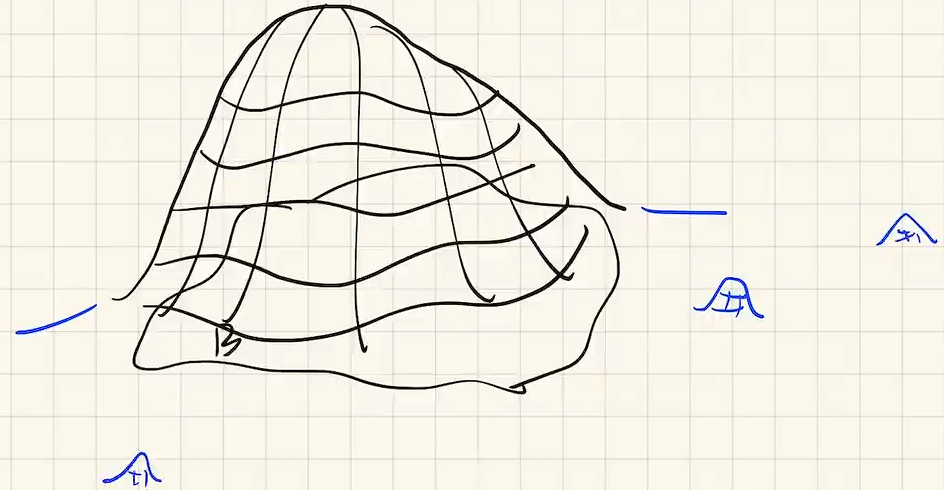
\includegraphics[width=0.65\linewidth]{figure/3.1.3-1}
 			\caption{Prop 3.1.6 (\rmnum{1})}
 			\label{pic : 3.1.3-1} % 添加图像引用标签
 		\end{minipage}
 		\begin{minipage}[t]{0.40\linewidth}
 			\centering
 			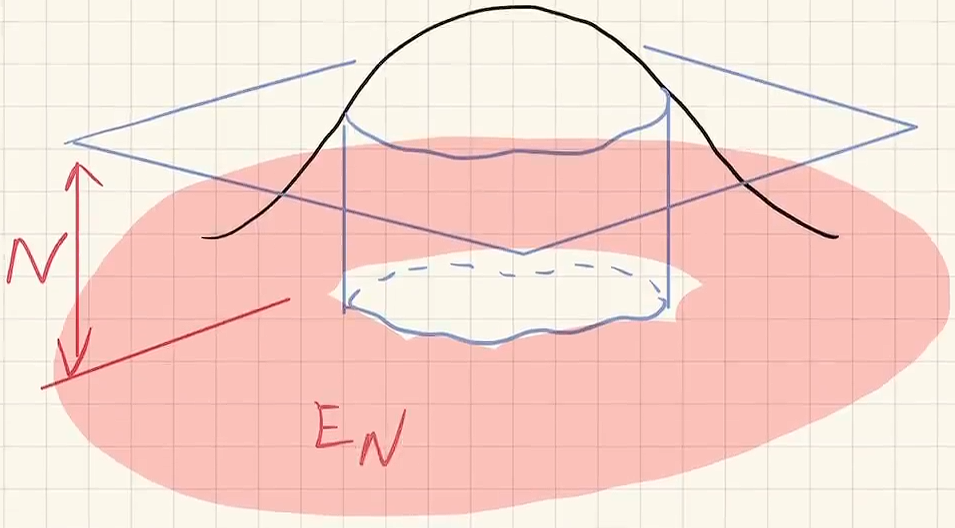
\includegraphics[width=0.65\linewidth]{figure/3.1.3-2}
 			\caption{Prop 3.1.6 (\rmnum{2})} % 添加图像标题
 			\label{pic : 3.1.3-2} % 添加图像引用标签
 		\end{minipage}
 	\end{figure}

 \newpage
 
 \subsection{$The \,\, Dominated \,\, Convergence \,\, Theorem$}
 	下面我们来介绍实分析中最最有用的定理——
 	\begin{center}
 		\underline{\textbf{控制收敛定理 (The Dominated Convergence Theorem)}}.
 	\end{center}
 	
 	\vspace{2em}
 	在\textbf{Riemann 积分}中,对于函数列\textbf{交换极限与积分的次序}的条件太过于奇怪与繁琐,而在\textbf{Lebesgue 积分}中,\textbf{控制收敛定理}则很完美地解决了这一问题. 它对于\textbf{交换极限与积分的次序}的条件十分简洁.下面便来介绍这一定理.
 	\begin{thm}\label{thm 3.1.7}
 		\textbf{The Dominated Convergence Theorem (DCT)}. \\
 		Suppose $\{ f_n \}_{n = 1}^{\infty} \subset \mathcal{M}^{+}$, $f_n \rightarrow f$ a.e.. If $\left| f_n \right| \leq g$, where $g \in \mathcal{L}^{1}(\R^d)$, then
 		\begin{align}
 			\int{\left| f_n - f \right|} \to 0 , \,\, n \to \infty
 		\end{align}
 		and consequently
 		\begin{align}
 			\int{f_n} \to \int{f} , \,\, n \to \infty
 		\end{align}
 	
 		\vspace{3em}
 		\begin{proof}
 			分别对$g + f_n$ 和$g - f_n$ 利用\textbf{Fatou's Lemma (Thm \ref{thm 3.1.6})}即可得证.
 			\begin{itemize}
 				\item Since $g + f_n \geq 0$, then by \textbf{Fatou's Lemma (Thm \ref{thm 3.1.6})},
 				\begin{align}
 					\int{\liminf_{n \to \infty}{(g + f_n)}} \leq \liminf_{n \to \infty}{\int{(g + f_n)}} 
 				\end{align}
 				Since $f_n \to f$, we have
 				\begin{align}
 					\int{g} + \int{f} &\leq \int{g} + \liminf_{n \to \infty}{\int{f_n}} \\
 					\int{f} &\leq \liminf_{n \to \infty}{\int{f_n}}
 				\end{align}
 				
 				\vspace{1em}
 				
 				\item Since $g - f_n \geq 0$, then by \textbf{Fatou's Lemma (Thm \ref{thm 3.1.6})},
 				\begin{align}
 					\int{\liminf_{n \to \infty}{(g - f_n)}} &\leq \liminf_{n \to \infty}{\int{(g - f_n)}} \\
 					\int{g} - \int{f} &\leq \int{g} + \liminf_{n \to \infty}{(-\int{f_n})} \\
 					&= \int{g} - \limsup_{n \to \infty}{\int{f_n}}
 				\end{align}
 				Then
 				\begin{align}
 					\int{f} \geq \limsup_{n \to \infty}{\int{f_n}}
 				\end{align}
 			\end{itemize}
 			Therefore
 			\begin{align}
 				\limsup_{n \to \infty}{\int{f_n}} \leq \int{f} \leq \liminf_{n \to \infty}{\int{f_n}}
 			\end{align}
 			which means $\underset{n \to \infty}{\lim}{\int{f_n}}$ exists, and
 			\begin{align}
 				\lim_{n \to \infty}{\int{f_n}} = \int{f}
 			\end{align}
 		\end{proof}
 	\end{thm}
 
 \newpage
 \subsection{$Complex-Valued \,\, Functions$}
 \begin{center}
 	下面我们将\textbf{实值函数}上的\textbf{Lebesgue 积分}推广至\textbf{复值函数}.
 \end{center}
 	
 	先来规定一些记号:
 	\begin{itemize}
 		\item Let $f : \R^d \rightarrow \C$, write $f(x) = u(x) + i v(x)$.
 	\end{itemize}
 	
 	\vspace{2em}
 	下面给出复值函数\textbf{可测}以及\textbf{可积}的定义.
 	\begin{defn}\label{def 3.1.7}
 		Suppose $f : \R^d \rightarrow \C$, $f = u + iv$, then we say
 		\begin{itemize}
 			\item $f$ is \underline{\textcolor{blue}{\textbf{measurable}}} if $u$ and $v$ are both measurable.
 			
 			\item $f$ is \underline{\textcolor{blue}{\textbf{Lebesgue integrable}}} if $\left| f \right|$ is Lebesgue integrable.
 		\end{itemize}
 		
 		\vspace{2em}
 		\begin{rmk}
 			事实上,根据此处定义,$f$ 可积 $\,\, \Leftrightarrow \,\,$ $u$ and $v$ 都可积.
 			\begin{proof}
 				\begin{itemize}
 					\item $f$ is integrable $\,\, \Rightarrow \,\,$ $\int{\sqrt{u^2 + v^2}} < \infty$ $\,\, \Rightarrow \,\,$ $\int{\left| u \right|} , \int{\left| v \right|} \leq \int{\sqrt{u^2 + v^2}} < \infty$ $\,\, \Rightarrow \,\,$ $u$ and $v$ 可积.
 					
 					\item $u$ and $v$ 可积 $\,\, \Rightarrow \,\,$ $\int{\left| u \right|} , \int{\left| v \right|} < \infty$ $\,\, \Rightarrow \,\,$ $\int{\sqrt{u^2 + v^2}} \leq \int{\left| u \right|} + \int{\left| v \right|} < \infty$ $\,\, \Rightarrow \,\,$ $f$ 可积.
 				\end{itemize}
 			\end{proof}
 		\end{rmk}
 	\end{defn}
 	
 	\vspace{2em}
 	下面对\textbf{命题 \ref{prop 3.1.5}} 的结论进行推广,即由\textbf{复值可积函数}构成的空间为\textbf{线性空间}.
 	\begin{proposition}\label{prop 3.1.7}
 		$\mathcal{L}^{1}(\R^d , \C)$ is a vector space.
 		
 		\vspace{2em}
 		\begin{proof}
 			Trivial.
 		\end{proof}
 	\end{proposition}
 
 
 \newpage
 
\section{$\mathcal{L}^1$ 空间的完备性}
\paragraph{引入}
	在讲\textbf{Riemann积分}时,我们称\textbf{Riemann可积函数}构成的空间是\textbf{不完备的 (not complete)}. 在提及\textbf{完备}这个概念之前,我们需要先引入衡量“距离”的工具,即\textbf{范数}和\textbf{度量}.
	
	\vspace{2em}
	\subsection{范数,度量}
 	下面给出\textbf{范数}和\textbf{度量}的严格定义.
 	\begin{defn}\label{def 3.2.1}
 		Let $X$ be a vector space over $\mathbb{F}$, a \underline{\textcolor{blue}{\textbf{norm}}} is a function:
 		\begin{align}
 			X &\longrightarrow \R_{\geq 0} \\
 			f &\longmapsto \Vert f \Vert
 		\end{align}
 		satisfying the following properties:
 		\begin{enumerate}
 			\item[(\rmnum{1})]$\Vert f \Vert \geq 0$, $\forall f \in X$. \hspace*{3em} ($\Vert f \Vert = 0 \,\, \Leftrightarrow \,\, f = 0 \,\, a.e.$)
 			
 			\item[(\rmnum{2})]$\Vert af \Vert = \left| a \right| \Vert f \Vert$, $\forall a \in \mathbb{F}, f \in X$.
 			
 			\item[(\rmnum{3})]$\Vert f + g \vert \leq \Vert f \Vert + \Vert g \Vert$, $\forall f , g \in X$.
 		\end{enumerate}
 		
 		\vspace{2em}
 		\begin{rmk}
 			\begin{itemize}
 				\item (\rmnum{1})中的“$\Vert f \Vert = 0 \,\, \Leftrightarrow \,\, f = 0 \,\, a.e.$”的\textbf{“a.e.”}是对于$X$ 取函数空间时的条件,在实分析的取等条件中基本为默认叙述,在后续定义中往往省略. 在对$\mathcal{L}^1$ 空间的定义 (\textbf{定义 \ref{def 3.2.4}})中可以看到其合理性.
 				
 				\vspace{1em}
 				
 				\item \textbf{范数}实际上是对$\R^n$ 空间中\textbf{“与原点之间的距离”}这一概念的推广. 将函数视作向量,则其范数即为到原点的距离,即\textbf{模长}.
 				
 				\vspace{1em}
 				
 				\item 若一个\textbf{线性空间}$X$ 上配备了一个\textbf{范数},则称其为\textcolor{blue}{\textbf{赋范向量空间 (赋范线性空间)}}.
 			\end{itemize}
 		\end{rmk}
 	\end{defn}
 
 	\newpage
 	将函数视作向量,就有其\textbf{到原点的距离}为\textbf{范数}. 但若是想要衡量\textbf{任意两个函数之间的距离},则需要引入下面\textbf{度量}的概念.
 	\begin{defn}\label{def 3.2.2}
 		A \underline{\textcolor{blue}{\textbf{metric}}} on $X$ is a map
 		\begin{align}
 			d : X \times X &\longrightarrow \R_{\geq 0} \\
 			(x , y) &\longmapsto d(x , y)
 		\end{align}
 		satisfying
 		\begin{enumerate}
 			\item[(\rmnum{1})]$d(x,  y) \geq 0$, $\forall x , y \in X$. \hspace*{3em} ($d(x , y) = 0 \,\, \Leftrightarrow \,\, x = y$)
 			
 			\item[(\rmnum{2})]$d(x , y) = d(y , x)$, $\forall x , y \in X$.
 			
 			\item[(\rmnum{3})]$d(x , y) + d(y , z) \geq d(x , z)$, $\forall x , y , z \in X$.
 		\end{enumerate}
 		
 		\vspace{2em}
 		\begin{rmk}
 			\begin{itemize}
 				\item 若$X$ 为函数空间,则 (\rmnum{1})中“$d(x , y) = 0$”等价条件默认为“$x = y \,\, a.e.$”.
 				
 				\vspace{1em}
 				
 				\item \textbf{度量}可看作将两个函数 (向量)的起点均平移至原点后,其两个终点之间的\textbf{距离}.
 			\end{itemize}
 		\end{rmk}
 	\end{defn}
 
\vspace{2em}
\subsection{$The \,\, Space \,\, \mathcal{L}^{1}(\R^d)$}
\paragraph{范数}
	下面先在所有\textbf{Lebesgue可积函数}构成的空间上定义\textbf{范数}.
	\begin{defn}\label{def 3.2.3}
		For any integrable function $f$ on $\R^d$, we define the \underline{\textcolor{blue}{\textbf{norm}}} of $f$,
		\begin{align}
			\Vert f \Vert = \int_{\R^d}{\left| f \right| dx}
		\end{align}
	
		\vspace{1em}
		\begin{rmk}
			\begin{itemize}
				\item 由\textbf{命题 \ref{prop 3.1.3}}可知,此处$\Vert f \Vert = 0 \,\, \Leftrightarrow \,\, f = 0 \,\, a.e.$
				
				\vspace{1em}
				
				\item 容易证明,如此定义的\textbf{范数}满足范数应当满足的三条公理. (\textbf{定义 \ref{def 3.2.1}})
			\end{itemize}
		\end{rmk}
	\end{defn}

\newpage
\paragraph{\textbf{Space $\mathcal{L}^{1}(\R^d)$}}
	由于\textbf{定义 \ref{def 3.2.3}}中“$\Vert f \Vert = 0 \,\, \Leftrightarrow \,\, f = 0 \,\, a.e.$”,而我们对零测集上的函数性质并不关心,因而引出了如下关于$\mathcal{L}^1$ 空间的定义.
	\begin{defn}\label{def 3.2.4}
		我们在所有\textbf{Lebesgue可积函数}构成的空间上定义一个等价关系“$\sim$”:
		\begin{center}
			$f \sim g \,\, \Leftrightarrow \,\, f = g \,\, a.e.$
		\end{center}
		\textcolor{blue}{$\mathcal{L}^{1}(\R^d)$} is \underline{\textcolor{blue}{\textbf{the space of equivalences classes}}} of integrable functions.
		
		\vspace{2em}
		\begin{rmk}
			由定义可知,$\mathcal{L}^{1}(\R^d)$ 空间中的元素实际上为\textbf{函数的等价类 (集合)}
			\begin{center}
				$[f] = \{ g \,\, integrable \mid g \sim f \}$
			\end{center}
			而在实际中,我们还是习惯性地当作单独的函数进行运算,这在\textbf{几乎处处}的意义下时等价的.
		\end{rmk}
	\end{defn}

\vspace{2em}
\paragraph{度量}
	下面我们说明,根据\textbf{定义 \ref{def 3.2.3}} 中所定义的\textbf{范数}可诱导出$\mathcal{L}^{1}(\R^d)$ 上的一个\textbf{度量}.
	
	\begin{proposition}\label{prop 3.2.1}
		\begin{align}
			d : \mathcal{L}^{1}(\R^d) \times \mathcal{L}^{1}(\R^d) &\longrightarrow \R_{\geq 0} \\
			(f , g) &\longmapsto d(f , g) \coloneqq \Vert f - g \Vert
		\end{align}
		defines a \underline{\textcolor{blue}{\textbf{metric}}} on $\mathcal{L}^{1}(\R^d)$.
		
		\vspace{2em}
		\begin{proof}
			下面即来逐一验证\textbf{定义 \ref{def 3.2.2}} 中的三条公理.
			\begin{itemize}
				\item 根据范数的非负性,$\forall f , g \in \mathcal{L}^{1}(\R^d)$,$d(f , g) = \Vert f - g \Vert \geq 0$.
				\begin{center}
					$d(f , g) = 0 \,\, \Leftrightarrow \,\, f - g = 0 \,\, a.e. \,\, \Leftrightarrow \,\, f = g \,\, in \,\, \mathcal{L}^{1}(\R^d)$
				\end{center}
			
				\item 可交换性. $\forall f , g \in \mathcal{L}^{1}(\R^d)$,
				\begin{align}
					d(f , g) = \vert f - g \Vert = \int_{\R^d}{\left| f - g \right|} = \int_{\R^d}{\left| g - f \right|} = \Vert g - f \Vert = d(g , f)
				\end{align}
			
				\item 根据范数的三角不等式,$\forall f, g , h \in \mathcal{L}^{1}(\R^d)$,
				\begin{center}
					$d(f , g) + d(g , h) = \Vert f - g \Vert + \Vert g - h \Vert \geq \Vert (f - g) + (g - h) \Vert = \Vert f - h \Vert = d(f , h)$
				\end{center}
			\end{itemize}
		\end{proof}
	\end{proposition}

\newpage
\subsection{$\mathcal{L}^1$ 空间的完备性}
\paragraph{定义}
	在得到了\textbf{范数}、\textbf{度量}的定义后,我们下面给出\textbf{完备空间}的定义.
	\begin{defn}\label{def 3.2.5}
		A \textbf{metric space} $X$ is \underline{\textcolor{blue}{\textbf{complete}}} if every Cauchy Sequence $\{ x_k \}_{k = 1}^{\infty}$ has a limit in $X$.
		
		\vspace{2em}
		\begin{rmk}
			\begin{itemize}
				\item \textbf{完备空间}即指空间中的任一柯西列都有\textbf{收敛到自身}的极限.
				
				\vspace{1em}
				
				\item 下面给出一个\textbf{不完备的度量空间}的例子.
				\begin{example}\label{ex 3.2.1}
					取一维实数域$\R$ 的子空间$(0 , 1) \subset \R$,考虑其上的Cauchy Sequence $\{ \frac{1}{n} \}_{n = 2}^{\infty} \subset (0 , 1)$.\\
					由于$\frac{1}{n} \to 0 \notin (0 , 1)$,因此度量空间$(0 , 1)$ 不完备.
				\end{example}
			\end{itemize}
		\end{rmk}
	\end{defn}

\vspace{2em}
\paragraph{\textbf{$\mathcal{L}^1$ 空间的完备性}}
	下面我们将给出本小节最重要的结论,即$\mathcal{L}^1$ 空间的\textbf{完备性},这也是其比\textbf{Riemann可积函数}所构成的空间的优越性之所在.
	
	\begin{thm}\label{thm 3.2.1}
		\textbf{(Riesz - Fischer)}. 
		\begin{center}
			$\mathcal{L}^1$ is complete in its metric.
		\end{center}
	
		\vspace{2em}
		\begin{proof}
			Let $\{ f_n \}_{n = 1}^{\infty} \subset \mathcal{L}^{1}(\R^d)$ be a Cauchy Sequence in $\mathcal{L}^1$, then
			\begin{center}
				$\forall \epsilon > 0$, $\exists N(\epsilon) \in \N$, $\forall n , m \geq N(\epsilon)$, $\st \Vert f_n - f_m \Vert \leq \epsilon$
			\end{center}
			Tacking $\epsilon = 2^{-k}$, then $\exists N(2^{-k}) \geq N^{2^{-(k - 1)}}$, $\st$ for $n_k = N(2^{-k}) , n_{k + 1} = N(2^{-(k + 1)})$,
			\begin{center}
				$\Vert f_{n_k} - f_{n_{k + 1}} \Vert \leq 2^{-k}$
			\end{center}
			下面分为三步进行证明.
			\begin{itemize}
				\item 构建$f(x)$ 并利用$g(x)$ 证明$f \in \mathcal{L}^1$,证明子列$\{ f_{n_j} \}_{j = 1}^{\infty}$ 收敛到$f$. \\
				Let 
				\begin{align}
					f &= f_{n_1} + \sum_{j = 1}^{\infty}{(f_{n_{j + 1}} - f_{n_j})} \\
					g &= \left| f_{n_1} \right| + \sum_{j = 1}^{\infty}{\left| f_{n_{j + 1}} - f_{n_j} \right|}
				\end{align}
				Then by \textbf{MCT (Thm \ref{thm 3.1.2}, 控制收敛定理)}
				\begin{align}
					\int{g}
					= \int{\left| f_{n_1} \right|} + \int{\sum_{j = 1}^{\infty}{\left| f_{n_{j + 1}} - f_{n_j} \right|}}
					&= \int{\left| f_{n_1} \right|} + \sum_{j = 1}^{\infty}{\int{\left| f_{n_{j + 1}} - f_{n_j} \right|}} \\
					&= \int{\left| f_{n_1} \right|} + \sum_{j = 1}^{\infty}{\Vert f_{n_{j + 1}} - f_{n_j} \Vert} \\
					&\leq \int{\left| f_{n_1} \right|} + \sum_{j = 1}^{\infty}{2^{-j}}
					< \infty
				\end{align}
				Therefore $g$ is integrable, $g \in \mathcal{L}^1$. Since $\left| f \right| \leq g$, then $\int{\left| f \right|} < \infty$. $f$ is integrable. \\
				Let
				\begin{align}
					S_{k} = f_{n_1} + \sum_{j = 1}^{k}{(f_{n_{j + 1}} - f_{n_j})} = f_{n_{k + 1}} , \,\, k = 1 , 2 , \cdots
				\end{align}
				\begin{center}
					$f$ is integrable $\,\, \Rightarrow \,\,$ $f < \infty \,\, a.e.$ $\,\, \Rightarrow \,\,$ $S_k$ converges a.e. $\,\, \Rightarrow \,\,$ $S_k = f_{n_{k + 1}} \to f \,\, a.e.$
				\end{center}
				So we find
				\begin{center}
					$f_{n_k} \to f \,\, a.e.$
				\end{center}
				
				\vspace{4em}
				\item 将逐点收敛性转化为$\mathcal{L}^1$ 收敛性,即证$\Vert f - f_{n_k} \Vert \to 0$. \\
				We note that
				\begin{align}
					\left| f - f_{n_k} \right|
					&= \left| \left( f_{n_1} + \sum_{j = 1}^{\infty}{(f_{n_{j + 1}} - f_{n_j})} \right) - \left( f_{n_1} + \sum_{j = 1}^{k - 1}{(f_{n_{j + 1}} - f_{n_j})} \right) \right| \\
					&=\left| \sum_{j = k}^{\infty}{(f_{n_{j + 1}} - f_{n_j})} \right| 
					\leq g
				\end{align}
				By \textbf{DCT (Thm \ref{thm 3.1.7}, 控制收敛定理)}, since $\left| f - f_{n_k} \right| \to 0 \,\, a.e.$, $\left| f - f_{n_k} \right| \leq g$, $g$ integrable,
				\begin{align}
					\lim_{k \to \infty}{\Vert f - f_{n_k} \Vert}
					= \lim_{k \to \infty}{\int{\left| f - f_{n_k} \right|}}
					\overset{\textbf{DCT}}{=} \int{\lim_{k \to \infty}{\left| f - f_{n_k} \right|}}
					= 0
				\end{align}
				Therefore, $\Vert f - f_{n_k} \Vert \to 0$. 即$f_{n_k}$ 依$\mathcal{L}^1$ 范数收敛到$f$.
				
				\newpage
				\item 利用子列$\{ f_{n_k} \}_{k = 1}^{\infty}$ 作为“桥梁”,证明$f_n$ 依$\mathcal{L}^1$ 范数收敛到$f$,即$\Vert f_n - f \Vert \to 0$. \\
				$\forall \epsilon > 0$,由于$\{ f_n \}_{n = 1}^{\infty}$ 为$\mathcal{L}^1$ 中Cauchy Sequence, 因此$\exists N \in \N$, $\st$
				\begin{center}
					$\Vert f_n - f_m \Vert < \frac{\epsilon}{2} , \,\, \forall n , m > N$
				\end{center}
				Since $\Vert f_{n_k} - f \Vert \to 0$, then for $\epsilon > 0$, pick $n_k > N$ which $\st$
				\begin{center}
					$\Vert f_{n_k} - f \Vert < \frac{\epsilon}{2}$
				\end{center}
				Then
				\begin{align}
					\Vert f_n - f \Vert 
					\leq \Vert f_n - f_{n_k} \Vert + \Vert f_{n_k} - f \Vert
					< \epsilon , \,\, \forall n > n_k > N
				\end{align}
				Therefore $\Vert f_n \to f \Vert \to 0$ with $f \in \mathcal{L}^1$. $\mathcal{L}^1$ is complete in its metric.
			\end{itemize}
		\end{proof}
	\end{thm}

	\vspace{2em}
	根据上述定理的证明过程,可以得到下面的推论.
	\begin{corollary}\label{cor 3.2.2}
		If $\{ f_n \}_{n = 1}^{\infty}$ converges to $f$ in $\mathcal{L}^1$, then there exists a subsequence $\{ f_{n_k} \}_{k = 1}^{\infty}$ such that
		\begin{center}
			$f_{n_k}(x) \to f(x) \,\, a.e.$
		\end{center}
	
		\vspace{1em}
		\begin{rmk}
			即在\textbf{依$\mathcal{L}^1$ 范数收敛}的函数序列中,总存在\textbf{“几乎处处收敛”}意义的子列.
		\end{rmk}
	\end{corollary}


	%  ############################
	\ifx\allfiles\undefined
\end{document}
\fi